\documentclass{article}

%-------------------------------------------------------------------------------
% TODO general list
%-------------------------------------------------------------------------------
% - 

%-------------------------------------------------------------------------------
% Imports
%-------------------------------------------------------------------------------
\usepackage{amsmath}
\usepackage{amssymb}
\usepackage{geometry}
\usepackage{graphicx}
\usepackage{etoolbox} % block quotes
\usepackage{setspace} % linespacing
\usepackage{xcolor}
\usepackage[nottoc,other]{tocbibind}

%-------------------------------------------------------------------------------
% Settings
%-------------------------------------------------------------------------------
\onehalfspacing
\AtBeginEnvironment{abstract}{\onehalfspacing}
\AtBeginEnvironment{quote}{\singlespacing}
\renewcommand{\tocbibname}{}

\graphicspath{ {./images/} }

\definecolor{linkcolor}{rgb}{0.0, 0.7, 0.5}
\usepackage[colorlinks, allcolors=linkcolor]{hyperref} % citation hyperlinks

%-------------------------------------------------------------------------------
% Commands
%-------------------------------------------------------------------------------
\newcommand{\tx}[1]{\text{#1}}
\newcommand{\ti}[1]{\textit{#1}}
\newcommand{\tb}[1]{\textbf{#1}}
\newcommand{\p}{^\prime}

% citations
\renewcommand{\cite}[1]{\hyperlink{#1}{#1}}
\newcommand{\reference}[3]{\bibitem{#1} \hypertarget{#1}{} #1. \ti{#2}. #3.}

% annotated bibliography
\newcommand{\annbibtitle}[2]{\subsection*{#1. \ti{#2}}}

\begin{document} % +===+===+===+===+===+===+===+===+===+===+===+===+===+===+

%-------------------------------------------------------------------------------
% Title
%-------------------------------------------------------------------------------
\begin{center}
	\huge{\bf Procession: Weak Emergence} % paper title
    \\[0.75cm] 
	\large{Henry Blanchette} % paper author
    \\[0.5cm]
	\large{Metaphysics of Science \\ Reed College} % paper organization
    \\[1.0cm]
\end{center}

%-------------------------------------------------------------------------------
% Abstract
%-------------------------------------------------------------------------------
\begin{abstract}
	Problems with accepting a layering of reality via some manner of non-reductive emergence turn out to stem not from a specific conception of emergence but rather from the non-specificity of most conceptions of emergence so far considered. Any bet on emergence being \ti{real} or \ti{unreal} should be refunded. I argue that a specification of emergence as process-centric, causally efficacious, and ontologically-novel both nearly addresses the causal overdetermination, downward-causation and epistemic-not-ontological arguments against such strong emergentism, as well as explains its own development.
\end{abstract}

\section{Concepts of Emergence}

``Emergence'' means as mysterious as it seems. The goal of this paper is to engage with the idea of in a top-down approach, by progressively increasing the technicality of what I mean when I write ``emergence'' (often with the help of some preceeding adjectives). So, for example in the Concepts of Emergence section when I talk about emergence very generally, I am intentionally leaving the specifications of what such a reference could entail as undecided and open. From the start, I attempt to assume the minimum of what comes to a reader's mind when they read ``emergence.''

My goal is \ti{not} to redefine ``emergence'' from the start and then show that when others use the same word they have subtly violated my definition. Definitions will prove important in theory I use to narrow what \ti{kind} of emergence I mean, but the specification of ``emergence'' in the first place I will take as a primarily empirical investigation.

% TOPIC: history of specifying emergence
% explain British Emergentist situation
% be general, and leave the following concepts ambiguous: ontological, epistemological, strong, weak.

In colloqial use, ``emergence'' describes the result, often a pattern, in a complexity that is simple to explain in an abstract but informal. The concept has been used in all sorts of literature, but can this term be put to important theoretical use? The brief bloom of the British Emergentists illustrate an attempt at this endeavor in a legitimately novel circumstance very relevant to science and philosophy.

In the middle of the 20th century, a popular and concerning problem was that of explaining all of chemical bonding in terms of newly-acclaimed and hugely successful physical theories. The expectation was that it should be possible, since the theories described the entirety of the observed relevant features of the participants of chemical bonding. Nevertheless, the physical theories were innaccurate.

There are two directions a conjectured (at the time) solution could take:
\begin{enumerate}
\item
    The physical theories do not take into account more fundamental properties relevant the interaction of atoms. (\ti{downward appeal})
\item
    The physical theories do not take into account chemical properties that only apply to the interactions of atoms and are not derived from physical properties of atoms i.e. mass, charge, etc. (\ti{upward appeal})
\end{enumerate}

I name them as the \ti{downward appeal} and the \ti{upward appeal} to bring into focuss what is unique about this instance of applying the British Emergentist idea. The downward appeal is intuitive, as it almost-monotonically describes the direction of physics for the entirety of its scientific history. But at this point in the 20th century, the upward appeal gained some reasonable empirical evidence. Experiment after experiment, it was starting to seem like a purely chemical theory of bonding --- one that explicitly rejected derivation from physics --- would be the only option left that would maintain the physical theories that were so rebustly correct in almost every other prediction so far. What is novel here is that the physical theory came first, and then the upward appeal came second, as apposed to the historic direction of such invenstigation.

What would be the implications of the upward appeal, should it turn out to be correct? As the British Emergentists held, it would stratiy reality into some sort of hierarchy. One level of the hierarchy would be \ti{the physical}, and another, higher, layer would be \ti{the chemical}. The higher-lower relationship characterizes that chemical things consist of physical things. But the key distinctiveness between the layers of the hierarchy is that each layer has its own set of natural laws. It might be that some laws apply at multiple layers, but it is a least possible for some layers to have laws that some other layers do not i.e. some chemical laws about bonding do not apply to the physical. This hierarchy was projected to extend to other fields of study as well, where the lowest level of the hierarchy is typically referred to as ``physics'' without loss of generality should it turn out to be something more fundamental than physics that has not yet been explored. The levels above physics are reffered to as the \ti{special sciences} as they intuitively have an emergent character beyond physics. The ordering and seperation of the layers was not meant to be an empirical claim, but serves as a scheme for why it serves to be, at least, theoretically useful:
\[
    \cdots <
    \tx{ Physics } <
    \tx{ Chemistry } <
    \tx{ Biology } <
    \tx{ Psychology } <
    \tx{ Sociology } <
    \tx{ Political Science } <
    \cdots
\]

This grand scheme, however, was short-lived. Later on in the same centuty, physicists eventually developed a causally reductive, if not conceptually intuitive, explanation for chemical bonding in terms of quantum mechanics. Of course, this specific science is still young and under heavily development to this day, but as empirical evidence goes it was a desicive blow to the British Emergetist dogma in the eyes of the philisophical community. If the only empirical counterexample (and non-constructive at that) was overturned against British Emergentism, then there was little left to hold its sway. And though this specific strain of Emergentism has failed, it still has sparked and interest in some intriguing questions.

% other canonical examples of emergence
The example of chemical bonding was far from the only theoretical example of emergence as this tradition saw it. There were several other canonical examples, including conciousness, free will, life, and reproduction. The viewing of these phenomenon as emergent stemmed primarily from the colloqial sense of emergence this section behgan in reference to, but especially conciousness and free will have developed into large philosophical topics that increasingly beg for a specification of ``emergence''. Additionally, the somewhat unexpected reduction of quantum mechanics seems to shift at least some onus onto the naive emergentist to justify why the intuition for identifying emergence is correct, and that it is a concept beyond just explanatory vagueness.

% utility of the concept of emergence:
% - special sciences (Fodor)
% - features of explanations (Dennett)

But what of the hierarchy of studies that the British Emergentists postulated. The contention is of either allowing emergence, which allows laws for some levels in the hierarchy that are not derivable from laws of lower levels in the hierarchy, or disallowing emergence which should, in some way, make the hierarchy collapse on its lower level. It seems that in some ways of meaning ``emergence'', this contention is problematic. In other ways, perhaps it is not. \cite{Fodor J. A. 1974} describes a distinction between two sperspectives opposing emergence:

\begin{itemize}
    \item The \ti{Unity of Science} views that each science has as its fundamental aim the construction of a lowest-level-termed (i.e. physically-termed) explanation of its studyied phenomena
    \item The \ti{Generality of Physics} views that each instance of a phenomena studied by a science is completely explainable in lowest-level (i.e. physical) terms.
\end{itemize}

The problem with the Unity view is its implication that the more successful the special sciences are, the more reason there is to abandon them; the special sciences most commonly do not aim to reduce their explanations to physically-termed ones so to forward their projects is to drift further and further off into the clouds, away from a correct landing posisition on the solid, physical ground. This is a problem because it does not seem to match at all the history of progress in the special sciences very well well independent from physics. There is a wide range of ``closeness-to-physics'' over all special sciences, but there are obvious examples e.g. almost all social sciences. So, thus far we seem to have little reason to practice with the Unity claim.

On the other hand, the Generality view is much more in line with the endeavors of most scientists. The Generlity of Physics allows special scientists to forward explanations of phenomena in terms that they don't even dream to reduce to physics while still accepting that there is, somehow, a physical reduction of any phenomenon instance to which their explanation applies. In other words, all phenomena are physical in nature, but abstract explanations are nontheless useful.

What makes an explanation useful? They key question to answer is ``useful for what?''. \cite{Dennett D. C. 1991} illustrates two degrees of utility when it comes to explanations: accuracy and simplicity. These features generally trade-off, and over a variety of circumstances the valuation of one compared to the other can change. With this in mind, emergence seems most readily to yield explanations of simplicity over accuracy. Take for example the chemical bonding case, where we actually do have a lower-level explanation. Before the development of quantum mechanical explanations, chemists had a theory of chemical bonding in exclusively chemical terms. One motivation for developing a physical theory was that the chemical theory had exceptions --- it lacked precision --- and of course a physical theory should have obsolute precision. Yet, while the quantum mechanical theory of chemical bonding is universal accepted throughout the chemistry community today, chemists still often use the chemistry-termed theories for their (relative) simplicity among other reasons.

% TODO: talk about bar code maybe
\begin{figure}[h]
\centering
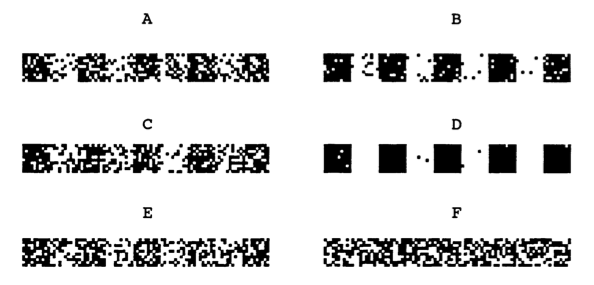
\includegraphics[width=8cm]{barcode}
\end{figure}

\section{Epistomological and Ontological Considerations}

% how emergence could be all in the mind

The considerations ending the previous section provoke an important test for any specification of emergence: ``is emergence just in the mind?'' If something seems emergent in light of an explanation that, for example, trades precision for simplicity (as would be claimed if one decided that chemical bonding was truely emergent from atomic interactions), then a thing's being emergent is not a property of the thing itself - it is in the eye of of the explainer. If this epistomological basis for emergence is accepted, then the project of specifying ``emergence'' devolves into a study of how humans prefer explanations and how they first come to explain somewhat complex phenomena before learning the real \ti{true} behind.

% TODO: talk about Searle's suggestion that we account for emergence just by redefining terms especially vis a vis consciousness. this concern though can be worked around by a gradually-narrowing specification of emergence as I practice in this paper

Although the described project would interseting to explore, it is certainly a concession of the original \ti{feel} of ``emergence''. If to be ``emergent'' is just to be crudely explained (where a crude explanation may still be useful), then emergence does not have metaphysical substance, which was clearly the driving force behind the canonical examples of applying emergence to consciousness, free will, etc. Obviously we do not have a physically-reductive explanation of either, and it is not unlikely that we might never, but is to assume that one does exist an act of epistemic humility or the opposite? And is to appeal to emergence an act of arrogance?

Both \cite{Wilson J. 2018} and \cite{Bedau M. 2018} agree that two central precepts for emergence are

\begin{enumerate}
\item Emergent phenomena are \ti{dependent} on underlying, lower-level processes.
\item Emergent phenomena are \ti{autonomous} from underlying lower-level processes.
\end{enumerate}

In what way emergent phenomena are so dependent and autonomous is the crux for determining their metaphysical status, and on this Wilson and Bedau diverge. Bedau claims that emergent phenomena are causally autonomous from and ontologically dependent on underlying lower-level processes. Wilson agrees that emergent phenomena are causally autonomous from underlying lower-level processes, but finds issue with allowing them to be ontologically dependent, and thus ontologically reducible to, underlying lower-level processes. Wilson argues that causal autonomy and ontological reducibility are incompatible. If refering to the whole is the same as referring to a conglomeration, in some way, of the parts, then how can the whole's causations be autonomous from the causations of its parts? Wilson has a solution (and different approach altogether) to this problem which I will discuss in section 3.

As for now, Bedau's view requires an explanation for how to specify an objective, mind-independent, definition for emergence that fits his qualifiations above. He gives the following definition:

\begin{quote}
If $P$ is a macro-property of some system $S$, then $P$ is Weakly emergent if and only if $P$ is \ti{generatively explainable} from all $S$'s prior micro-facts but only in an incompressible way.
(\cite{Bedau M. 2008})
\end{quote}

I will address specifically the idea of Weak as opposed to Strong emergence in section 3. 
I will reference just emergence generally, which includes Weak emergence of coures, and go into the detailed distinctions later. The definition of ``generatively explainable'' is

\begin{quote}
A \ti{generative explanation} of a macro-state is one that exactly and correctly explains how macro-events unfold over time - how they are generated dynamically.
(\cite{Bedau M. 2008})
\end{quote}

So to claim that a higher-level property $P$ is emergent from some lower levels properties $S$ is to claim that (a) there is an incompressible, generative explanation for $P$ in terms of $S$, and (b) there is not any compressible, generative explanation for $P$ in terms of $S$. Bedau defines \ti{compressible} as

\begin{quote}
If an explanation is \ti{compressible}, then explaining the macro-property abitrarily far into the future takes some fixed and finite amount of explanatory effort, not matter how far int othe future your explanation reaches.
(\cite{Bedau M. 2008})
\end{quote}

Proving that there is no compressible, generative explanation for some emergent property in nature, such as conciousness or free will, seems to be an extremeley difficult task. In fact, a negative proof is probably impossible, so finding indirect evidence is likely the best way to make progress on those fronts, under this view of emergence. But a certain recently-developed source of examples provides a constructive case for viewing emergence in terms of explanatory compressibility: discrete simulation (most commonly via computer).

% TODO: game of life example figs
% some good ones: https://copy.sh/life/?pattern=13enginecordership

% \begin{figure}[h]
% \centering
% 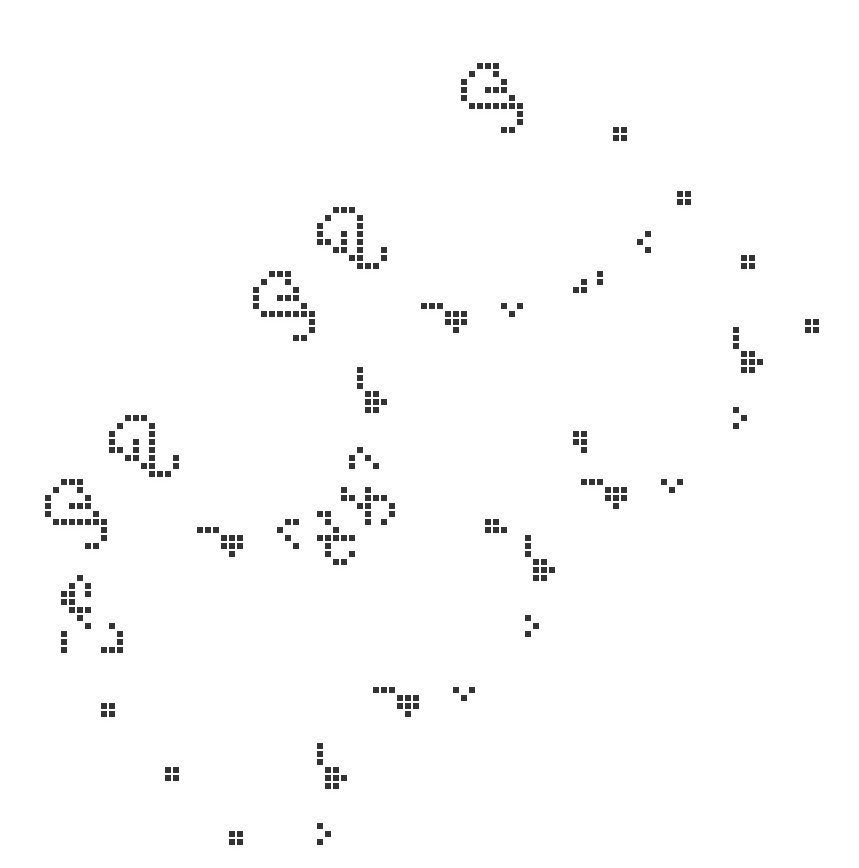
\includegraphics[width=9cm]{gol01}
% \end{figure}

% TODO: rather than use Game of Life, use cellular automata that I create myself

The most well-known implementation is John Conway's Game of Life, but any discrete simulation works in fundametally the same way:

\begin{enumerate}
\item The simulation is designed with a unambiguous, unchanging Rule. The Rule takes as input a State and gives as output a State, where a State is a full description of everything about the simulation other than the Rule.
\item To start running the simulation, it is given a initial State as its current State.
\item Then, the simulation applies its Rule to the current State and sets its current State to be the result. This completion of one iteration of this step is counted as one \ti{generation} of the simulation.
\item The simulation can be run for any finite number of generations.
\end{enumerate}

For the Game of Life simulation, the State is a 2-dimensional grid containing boolean values (referred to as cells and usually represented by pixels). The Rule describes what the value of each cell of a given State turns to, given the values of the 8 cells surrounding it. The Game of Life is one of a family of similar simulations called cellular automata. There are $2^{10}$ possible locally-ruled cellular automata that play out on a two-dimensional grid, of which the Game of Life is just one ($2^{10} = 2^9 \cdot 2$ is derived from the fact that to update a given cell a Rule takes into account the $9$ local cells' values (including the original cell itself), of which there are $2^9$ possible configurations, and then assigns a new value to the center cell, of which there are $2$ possibilities).

Conway's Game of Life is especially notably among all of these possibilities. An example of an uninteresting Rule is the one which assigns a cell to $0$ for any possible arrangement of its neighbors (the $0$-Rule). It is uninteresting because no matter the initial State, it is simple and obvious what every subsequent generation will look like. So, the Game of Life is somewhat special in producing the pretty life-like patterns that are its namesake; not just any rule could make those patterns.

Is the activity of the Game of Life any different, in an abstract sense, from the $0$-Rule? On the surface, it might seem like the generations of the Game of Life are harder to predict than the $0$-Rule, scaling in difficulty with the number of generations outward. The meaning of \ti{hardness} needs to be specified to make sense of this judgment. If hardness is taken to just be the difficulty for some particular explainer (such as a human mind) to generatively explain the simulation, then the resulting emergence is just a description of the relation between the proces and the simulation. This would mean that the appearance of emergence in the Game of Life and its lack in $0$-Rule is not necessarily inherent to the simulations themselves. Of couse, this implies that emergence is a purely epistomological concept. For emergence to apply metaphysically and not just to a relation between simulations and explainers, an objective measure of explanatory dfficulty must be specified to impose an order of compressibility on possible generative explanations. In what Bedau calls the \ti{complexity sciences}, several formal senses of computational complexity (i.e. hardness, difficulty) have been specified. An abstract specification of computational complexity is

\begin{quote}
\ti{Computation complexity}: the number of atomic steps, applied to facts of any level of generality about the simulation, required to exactly derive the resulting state of the simulation after some number $n$ generations, as a function of $n$.
\end{quote}

\ti{Atomic steps} are steps in a Turing machine where ``facts of any level of generality about the simulation'' are reprented by strings.

These new tools give a deeper insight into Bedau's specification of emergent phenomena as phenomena that are only generatively explainable in a incompressible way. An incompressible explanation is one that must run through the entirety of the lowest-level applications of the Rule (for each and every cell) for each successive generation, with no short-cuts. This grounds the inutition that $0$-Rule is uninteresting: we have a compressible generative explanation (as previously described), and with constant complexity at that. For the Game of Life, on the other hand, it has not been formally proven that there is not a compressible generative explanation, but it is almost universally conjectured that this is true.

% TODO: somewhere use the ``traffic jams are not just in the mind'' quote!

The application of emergence to these simulation examples is especially intriguing because not only do we have the lowest-level explanation for these phenomena, but we designed them and know everything about how they operate. If emergence can appear under these circumstances, then it seems plausible that just such emergence could occur in other seemingly-emergent cases. With the Game of Life, the emergent phenomenon is the activity of the computer that simulates it (executing the incompressible generative explanation), so this is cleary a real, non-hypothetical, example on hard silicon.

\section{Strong and Weak Emergence}

The definition of ``emergence'' as Bedau puts it, though strong in objectiveness, seems to be lacking in one of the original hallmarks of an emergent world: stratifying reality into a hierarchy. If to be emergent is to have a special arrangement of complexity, then is there really anything \ti{new} emerging? If the argument in the previous section that emergence is a metaphysical phenomenon and not just epistomological, then it is natural to expect emergence to add something to the ontology. \cite{Wilson J. 2018} chapter five expresses this concern with two prongs:

\begin{enumerate}
    \item[O1.] Metaphyisical autonomy is incompatible metaphysical (ontological and causal reducability), which Bedau claims to both hold of emeregence.
    \item[O2.] The causal powers of Bedau's emergent things are not distinguished from arbitrary disjunctions of the powers of the lower-level things on which the emergent thing depdends.
\end{enumerate}

% explain why talking about causal powers is important?

In fact, Bedau's definition seems to say little if anything about causal powers at all about causal powers. But what of this talk of powers? How and why are they important to this contention? Limiting or requiring causal powers is a dimension of anaylsis of the concept of emergence that has not yet been explicitly addressed. The first question to answer is ``what kind of \ti{things} does `emergence' apply to?'' \ti{Bedau M. 2008} poses that the atomic subject of emergence is the \ti{property}. Then, one can define an ``emergent entity'' to be ``an entity that has an emergent property.'', and an ``emergent phenomenon'' to be ``a phenomenon caused by entities with emergent properties.''

So when referencing the essence of emergence, we are focussing on the application of emergence to properties. This setup yields the direct link between emergence and causal powers, since the importance of properties is that entities have causal powers in regards to their properties; a property bestows some causal powers upon the entity which has it. This raises two important question about emergence:

\begin{enumerate}
    \item[Q1.] Is an emergent property an ontologically \ti{new} property?
    \item[Q2.] Does an emergent property bestow ontologically \ti{new} causal powers?
\end{enumerate}

For an emergent property to be ontologically \ti{new}, it needs to be distinct from any other property considered before realizing that there is this emergent property. The question can be rephrased, perhaps more intuitively, as ``when realizing that an entity is emergent do we attribute to the entity a new property, or does one of its old properties become emergent?'' This looks to be true, especially in light of Bedau's simulation examples from the previous section. 

\cite{Wilson J. 2018} goes into depth about causal details in her second chapter on Weak and Strong emergence.






% TODO: what do i even mean by this lol
\section{The Procession}

%-------------------------------------------------------------------------------
% Bibliography
%-------------------------------------------------------------------------------
% TODO: decide if newpage or not
\newpage
% TODO: order once all the entries are in
\section*{\centering References}
\begin{thebibliography}{11}

\bibitem{Bedau M. 2008} \hypertarget{Bedau M. 2008}{} Bedau M. 2008. Is Weak Emergence Just in the Mind? Minds and Machines 18:443–459. Springer.

\reference{Bedau M. 2018}{Downward Causation and the Autonomy of Weak Emergence}
    {Department of Philosophy at Reed College, OR USA}

\reference{Dennett D. C. 1991}{Real Patterns}
    {Reprinted in M. A. Bedau \& P. Humphreys (Eds.). (2008). \ti{Emergence: Contemporary readings in philosophy and science} (pp. 189-206). Cambridge: MIT Press}

\reference{Fodor J. A. 1974}{Special Sciences}
    {\ti{Synthese}, Vol. 28, No. 2 (Oct., 1974), pp. 97-115. Springer}

\reference{Hempel C., Oppenheim P. 1965}{On the Idea of Emergence}
    {Reprinted in M. A. Bedau \& P. Humphreys (Eds.). (2008). \ti{Emergence: Contemporary readings in philosophy and science} (pp. 61-68). Cambridge: MIT Press}

\reference{Humphreys P. 1997}{How Properties Emerge}
    {Reprinted in M. A. Bedau \& P. Humphreys (Eds.). (2008). \ti{Emergence: Contemporary readings in philosophy and science} (pp. 111-126). Cambridge: MIT Press}

\reference{McLaughin B. P. 1992}{The Rise and Fall of British Emergentism}
    {Reprinted in M. A. Bedau \& P. Humphreys (Eds.). (2008). \ti{Emergence: Contemporary readings in philosophy and science} (pp. 19-60). Cambridge: MIT Press}

\reference{McLaughin B. P. 1997}{Emergence and Supervenience}
    {Reprinted in M. A. Bedau \& P. Humphreys (Eds.). (2008). \ti{Emergence: Contemporary readings in philosophy and science} (pp. 81-98). Cambridge: MIT Press}

\reference{Searle J. 1992}{Reductionism and the Irredicibility of Conciousness}
    {Reprinted in M. A. Bedau \& P. Humphreys (Eds.). (2008). \ti{Emergence: Contemporary readings in philosophy and science} (pp. 61-68). Cambridge: MIT Press}

\reference{Wilson J. 2018}{Metaphysical Emergence}
    {Department of Philosophy at University of Toronto, ON CA}

\reference{Wolfram S. 1985}{Undecidability and Intractability in Theoretical Physics}
    {Physical Review Letters, Volume 54 Number 8. The American Physical Society}

\end{thebibliography}

%-------------------------------------------------------------------------------
% Annotated Bibliography
%-------------------------------------------------------------------------------
\newpage
\section*{\centering Annotated Bibliography}
\bigskip \bigskip

%-------------------------------------------------------------------------------
%-------------------------------------------------------------------------------
% TODO
\annbibtitle{Wilson J. 2018}{Metaphysical Emergence}
\subsubsection*{Chapter 1}

There are \ti{a priori} reasons for believing in emergenec, such as intuiting macro features while being aware of micro features. ``Hurricanes \dots trees \dots birts \dots and humans'' are commonly viewed emergent entites.

% NOTE: synchronic dependece, interseting to related to Bedau's observation
An observation: ``Accounts of emergence typically agree that core to the notion is the combination of synchronic meterial dependence and some form of autonomy.''

Notions of \ti{dependence}: ``Mereological (`part-whole') determination; Causation or nomological connection; Functional realization; Constitutive mechanism; The determinable-determinate relation; Inheritance of causal powers; Primitive `Grounding''

Notions of \ti{autonomy}: ``Nomological but not metaphysical supervenience; Non-fundamental novelty (of properties, powers, laws, entities); Fundamental novelty (of properties, powers, forces/interactions, laws, entities); non-additivity/non-linearity; ``Downward'' causal efficacy; Multiple realizability or compositional plasticity; Symmetry breaking; Elimination in degrees of freedom; The holding of a proper subset relation between token powers. “Epistemic criteria” notions include: In-principle failure of deducibility, predictability, or explicability; Predictability, but only by simulation; Lack of conceptual or representational entailment; theoretical/mathematical singularities.''

\smallskip
\noindent Kim's overdetermination argument:
\begin{enumerate}
    \item Dependence: Special science features depend on base features.
    \item Reality: Both of those things (special science features, base features) are real.
    \item Causal Efficacy: Special science features are causally efficacious.
    \item Distinctness: Special science features are distinct from their base features.
    \item Physical Causal Closure: For all low-level effects, there is a low-level cause.
    \item Non-Overdetermination: Effects are not at once caused by two sufficient causes.
\end{enumerate}

\noindent There are two instances of the problem:
\begin{enumerate}
    \item[I.] $S \rightsquigarrow S^*$ and $P \rightsquigarrow S^*$ (classical overdetermination)
    \item[II.] $S \rightsquigarrow P^*$ and $P \rightsquigarrow P^*$ (downward cuasation)
\end{enumerate}

\noindent Proposed solutions:
\begin{enumerate}
    \item Substance dualism or Pan/Proto-Psychism: $S, S^*$ do not respectively depend on $P, P^*$.
    \item Eliminativism: $S, S^*$ aren't real
    \item Epiphenomenalism: $S, S^*$ are not causally efficacious.
    \item Reductive physicalism: $S$ is not distinct from $P$.
    \item \tb{Strong emergentism}: Not every low-level effect has a low-level cause; deny $P \rightsquigarrow P^*$.
    \item \tb{Non-reductive physicalism}: Deny that overdetermination is problematic in a two-rock-throwing way.
\end{enumerate}

\tb{Strong emergentism} claims that some \ti{emergent features} has \ti{new powers} i.e. satisfies the \ti{new power condition}. The new power condition: Token higher-level feature S has, on a given occasion, at least one token power not identical with any token power of the token lower-level feature P on which S synchronically materially depends on that occasion.

Note that this denies physicalism.

\subsubsection*{Chapter 2}

This chapter focusses on \ti{Non-Reductive Physicalism}. NRP incorporates two conditions:

\begin{itemize}
    \item \ti{Token Identity of Powers Condition}: Every token power of an apparently higher-level feature​ $S$​, on a given occasion,is identical with a token power of a lower-level feature $P$​ ​on which $S$​ ​synchronically materially depends, on that occasion.
    \item \ti{Proper Subset of Powers Condition}: Token higher-level feature $S$ has, on a given occasion, a non-empty proper sibset of the token powers of hte token lower-level feature $P$ on which $S$ synchronically materially depends, on that occasion.
\end{itemize}

There are several ways to \ti{realize} the relationship between the realizers and the realized in emergenece compatible with NRP:

\begin{itemize}
    \item \ti{Functionalist}: realized types are higher-level types associated with causal roles that, on a given occasion, are played by tokens of realizer types. A causal role is just a collection of powers.
    \item \ti{Merelogical}: realized tokens or types are propert parts of base tokens or types respectively. This yields an emergence in the opposite direction of how it is typically concieved (parts are emergent from their wholes).
    \item \ti{Determinable/Determinate}: there is a relationship between type and token properties in terms of increasing specificity.
    \item \ti{Elimination in Degrees of Freedom}: An entity $E$ is Weakly (ontologically) emergent from some entities $e_i$ if (1) $E$ is composed of the $e_i$ as a result of imposing some constraints on the $e_i$ and (2) for some characteristic state $S$ of $E$ at least one of the DOF required to characterize a realizing system of $E$ as being in $S$ is eliminated from the DOF required to cahracterize $E$ as being in $S$.
\end{itemize}

The emergent properies' \ti{distinctive efficacy} is important to their metaphysical robustness. Leibniz's law yields that since realized properties have a proper subset of powers of their relizer properties, they cannot be identical, thus $S \neq P$. This counters reductive physicalism.

To address the problme of overdetermination and downward causation, Wilson shows some graphs that make use of the PSP relationship between the realized and the realizers. They conclude that never do we have to posit that some double-arrow is produced when there seems to only be room for one.

The schema for weak emergence is that $S$ and $P$ are both distinct and both causally efficacious. So, a higher-level feature $S$ is \tb{Weakly emergent} from lower level token features $P$ on a given occasion just in case, on that occasion, (1) $S$ synchronically materially depends on $P$, and (2) $S$ and $P$ satisfy the PSP condition.

Merricks has a slightly different overdetermination argument against emergence. It yields that for both the realizers and the realized properties to be causally efficacious, either one needs to cause the other to be efficacious or they are sufficiently efficatious only together. This argument cuts at Strong emergence, but doesn't seem to work on NRP.

\subsubsection*{Chapter 3}

Is consciousness strongly emergent? The \ti{physicalist} position is that mental states are identical to, or synchronically materially depend on, physical states.

The anti-physicalist knowledge argument:

\begin{enumerate}
\item[P0:] Mary has complete physics-knowledge of human color vision before her reslease.
\item[P1:] Mary has complete physical knwoledge about human color vision before her release.
\item[C1:] Therefore, Mary knows all the physical facts about human color vision, before her release.
\item[P2:] There is (some kind) of knowledge concerning facts about human color vision that Mary does not have before her release.
\item[C2:] Therefore, there are some facts about human color ivision that Mary does not know before her release.
\item[C3:] There are non-physical facts about human color vision (from C1, C2).
\end{enumerate}

Wilson's physicalist strategy to counter this argument is to say that
\[ \tx{Knowledge of Physics } \neq \tx{ Knowledge of the Physical} \]
where the Knowledge of the Physical is a subset of the Knowledge of the Mental.

The physicalist should maintain that:
\begin{enumerate}
\item Knowledge of the qualitative/subjective is physical knowledge.
\item And such knowledge can only be gained through acquaintance.
\item Therefore, contra P1, Mary cannot have complete physical knowledge before her release (from 1, 2).
\end{enumerate}

Conclusions:
\begin{quote}
Such an abstract, completely structuralist conception of the compositionally basic entities is not forced by physical theory. On the contrary: it is common for physicists to speak of particles or other lower-level physical phenomena as `feeling' forces, where the reference here might be thought to be both qualitative and sensitive to perspective—the force coming from this direction rather than that, and applied to the object in its location in ways that then enter into the object's moving in such-and-such a way. This degree of qualitativity, in which a non-complex physical entity is capable of registering a local perspective and associated sensitiv- ity to the environment, in a way that is not entirely qualitatively etiolated, clearly need not be seen as involving any measure of consciousness or mentality, even of a `protopsychic' variety. On the contrary, it reflects a naturalistic point of view according to which physical goings --- on are real and substantial, and when they move, they do so not because, e.g., they must play a predetermined part in the harmony of the spheres, but rather for some local salient reason or reasons --- i.e., one or more felt forces, or other form of interactive influence. This understanding of non-complex physical goings-on suggests that we should distinguish qualitativity and consciousness: sometimes these go together, as in creatures like us; but qualitativity is a weaker notion, that may be present, e.g., in the non-conscious response of a particle to the forces acting on it.
\end{quote}

\subsubsection*{Chapters 4 and 5}

This chapter focusses on complex systems. A complex system is a system that exhibits:
\begin{enumerate}
\item Nonlinearity
\item Extreme sensitiviy to internal conditions
\item Unpredictability
\item Algorithmic incompressibility (Bedau)
\item Universal behaviors
\item Self Organization
\end{enumerate}

Conway's Game of Life is a great case study of a complex system. The game is completely determined by its initial conditions and the subsequnt application of 4 rules on each micro-state each update. The result is a complex system (with all 6 characteristics) that is additionally Turing complete.

There arises a conflict between Wilson and Bedau's conceptions of Weak emergence.

\ti{Wilson's definition of Weak emergence}: Token apparently higher-level feature $S$ is weakly metaphysically emergent from token lower-level feature $P$ on a given occasion just in case, on that occasion, (i) $S$ synchronically materially depends on $P$, and (ii) $S$ has a non-empty proper subset of the token powers had by $P$.

\ti{Bedau's definition of Weak emergence}: Where $S$ is composed of micro-level entities having associated microstates, and where microdynamic $D$ governs the time evolution of $S$'s microstates: Macrostate $P$ of $S$ with microdyamic $D$ is weakly emergent if and only if $P$ can be derived from $D$ and $S$'s external conditions but only by simulation.

Wilson finds it odd that Bedau asserts that emergent phenomena are ontologically dependent on and reducible to micro phenomena.

Is Bedau's Weak emergence merely epistemological? No, because is an objective notion of existence about derivations of macrostates is metaphysical and not epistemological.

Wilson's objects to Bedau:
\begin{enumerate}
\item Incompatibility of metaphysical autonomy and metaphysical reducibility
\item Bedau hasn't said enough about causal powers of emergent powers and how to distinguish them from pointless disjunctions.
\end{enumerate}




%-------------------------------------------------------------------------------
%-------------------------------------------------------------------------------
\annbibtitle{Fodor J. A. 1974}{Special Sciences}

Consider and contrast two scientifically fundamental perspectives: the \ti{Unity of Science} and the \ti{Generality of Physics}. The Unity claim is actually stronger than the Generality claim; Unity of Science requires all sciences to have as their aim the construction of a physics-termed explanation of their studied phenomena, while Generality of Physics requires only that instances of studied phenomena be completely explainable in terms of physics. The Unity claim is, in fact, the central claim of Redictive Physicalism.

However, there is a seeming paradox in the Unity claim - it pronounces that the continued success of the special sciences is just more and more evidence that they ought to be discontinued; they stray further and further from an explanation in terms of physics. The \ti{special sciences} are sciences that do not deal directly or appeal to physical explanations.

\ti{Reductive Physicalism} is the view that all special sciences must reduce to physics. For some special-science relationship $S_1 \rightarrow S_2$, reductivism requires there be a reduction with to physical predicates $P_1, P_2$ such that

$$
\begin{array}{rcll}
    S_1 x & \rightarrow & S_2 x & \tx{(1)} \\
    S_1 x & \rightleftharpoons & P_1 x & \tx{(2a)} \\
    S_2 x & \rightleftharpoons & P_2 x & \tx{(2b)} \\
    P_1 x & \rightarrow & P_2 x & \tx{(3)}
\end{array}
$$

This setup forms a sort of bridge between the special-science relationship and a physical relationship. Though, there are some problems with the existence of bridges like this and how it interacts with the meaning of $\rightarrow$.

A way to address the bridge problems is with \ti{Token Physicalism}, where all events that the special sciences talk about are physical events.
\begin{itemize}
    \item Token physicalism is weaker than materialism, which claims token physicalism and that every event falls under the laws of some science or other.
    \item Token physicalism is weaker than type physicalism, where every property mentioned in the laws of any science is a physical property. This in fact implies token physicalism.
    \item Token physicalism is weaker than reductive physicalism, which claims token physicalism and that there are no natural kind predicates in an ideally completed physics which correspond ot each natural kind predicate in any ideally completed special science.
\end{itemize}

Every science implies a taxonomy of the events in its univers eof discourse. It creates theoretically- and empirically- inspired vocabulary, which fall under the laws of the science by virtue of satisfying those predicates. Not every theoretical predicate is valid or good though.

To fix reductive physicalism, can allow bridge relations to be in the form

$$
    S_x \leftrightharpoons P_1 x \lor \cdots \lor P_n x
$$

where $P_1 x \lor P_n x$ is not the kind of natural kind predicate in the reducing science. This allows for ``bridge laws'' to not really be laws, since they are not law-like. Reducing with this kind of bridge law looks like

$$
    P_1 x \lor \cdots \lor P_n x \leftrightharpoons P\p_1 \lor \cdots P\p_m
$$

Thesis:

\begin{quote}
There are special sciences not because of the nature of our epistemic relation to the world, but because of the way the world is put together: not all natural kinds (not all the classes of things and events about which there are important, counterfactual supporting generalizations to make) are, or correspond to, physical natural kinds.

A way of stating the classical reductionism view: things which belong to different physical kinds ipso facto can have no projectable descriptions in common; that if x and y differ in those descriptions by virtue of which they fall under the proper laws of physics, they must differ in those descriptions by virtue of which they fall under any laws at all.

If science is to be unified, then all such taxonomies must apply to the same things. If physics is to be basic science, then each of these things had better be a physical thing. But it is not further required that the taxonomies which the special sciences employ themselves reduce to the taxonomy of physics. It is not required, and it is probably not true.
\end{quote}

%-------------------------------------------------------------------------------
%-------------------------------------------------------------------------------
\annbibtitle{Bedau M. 2018}{Downward Causation and the Autonomy of Weak Emergence}

In this paper, Bedau explores a foundation of Weak emergence as \ti{derivability only by simulation} (or \ti{underivable except by simulation}).

The core precepts for the concept of emergence are:
\begin{enumerate}
    \item Emergent phenomena are dependent (ontologically) on underlying processes.
    \item Emergent phenomena are autonomous (causally) from underlying processes.
\end{enumerate}

All concepts of emergent base on the concept of the emergence property. The out-springing concepts include emergent entities (which are entities with emergent properties), emergent powers (which are powers bestowed by emergent properties), etc.

A property $P$ is underivable except by simulation if and only if $P$ can only be derived from a system, even a system causally closed at the lowest level, through a complete simulation of the low-level causes (e.g. \ti{gliders} in the Game of Life). Bedau poses that $P$ is Weakly emergent.

Basically, the idea is the if a property is interesting and complex in a formal way, in that it unpredictable arises from the low-level properties of a system, then it is indeed emergent (and, specifically, Weakly emergent).

It is important to note that this is a metaphysical point about emergent properties which is independent from epistemological concerns. For example, just because we haven't yet found a derivation sans simulation for a property doesn't mean that it is emergent - it just \ti{looks} emergent. Of course, a proof that there is not derivation is good, but such proofs are extremely hard to come by (especially because of the open $P =^? NP$ problem.)

Truely emergent properties are distinct from another kind of property that arises in similar circumstances - so-called \ti{resultant properties}. A property $P$ is a resultant property if and only if it is predictable from the properties of its parts. Often times, $P$ is just of a whole in and of itself and not an interesting emergence. $P$ of the whole that merely holds because of its being a whole as defined. For example, ``being a circle'' is a property that applies to a collection of points, but no single point in that collection shares the property of ``being a circle.'' However, this is uninteresting and is directly predictable from the definition of a circle and the properties of points, without having to do any sort of scaling computation to figure it out.


In the \ti{Game of Life}, there are many good examples of properties that are underivable except by simulation. For example, the property ``finitely-expanding.'' A worldstate that, after a finite number of time steps, reaches a maximum $m \times n$ area in the world such that no matter how many more time steps are run no cell will be born outside the area.

There are examples of non-finitely-expanding configurations, such as the famous \ti{Gospel Glider Gun} that creates gliders in intervals and sends them out into infinity. And there are examples of finitely-expanding configurations, such as any that consists of only non-interacting \ti{still-lifes}.

However, to derive if a worldstate is finitely-expanding, one needs to run a simulation. There is no general mathematical theorem that decides without doing the equivalent of a brute simulation. Even if a mega-computer could do the simulation instantaneous, it would still count as needing a simulation and thus ``finitely-expanding'' is an emergent property.

If, however, someone came up with a shortcut, it would prove that ``finitely-expanding'' is not emergent.

The main problem for emergence is that of \ti{downward causation} i.e. \ti{overdetermination}. If $S$ emerges from $P$ but $P$ is synchronically and ontologically dependent on $P$, then if $S$ causes a $P^*$ then surely we can say that $P$ causes $P^*$ as well. But if the low level of the $P$s is causally closed, then why do we need to talk about $S$ causing anything at all? It seems irrelevant and problematic in an overdeterminative way. But if $S$ was causally inefficacious, then it loses its status of autonomy from $P$ and is not really emergent in the first place. This is Kim's overdetermination argument.

But Kim's concerns are ill-founded. The idea of Weak emergence avoids the problems by yielding overdetermination as unproblematic, since it is causally reductionsitic and uses ontological dependence. But such weak emergence is important because it clearly defines autonomous and relevant structures.

Additionally, Weak emergence is not synchronic. It introduces a diachronic perspective on causation, where, for example, in the Game of Life for a macrostate to manifest an emergent property many time steps need to pass. For a microstate to have a property, it must be manifested in one or two time steps. In this case, emergent properties are causally relavant and distinct from lower-level properties.

Conclusion:
\begin{quote}
The advent of modern philosophy is conventionally presented as the Cartesian triumph over Aristotelian scholasticism. An Aristotelian thesis that attributed nature on the basis of a rich dependence on generating context was supplanted by the Cartesian antithesis that attributed reductionistic essences independent of context. Computer simulations allow weak emergence to extend reductionism into new territory, but they do so by embodying the idea that something's nature can depend on its genesis. Thus, the macro can depend on the context-sensitive process from which it arises and by which it is maintained. In this way, weak emergence can be viewed as a new synthesis.
\end{quote}

%-------------------------------------------------------------------------------
%-------------------------------------------------------------------------------
\annbibtitle{Bedau M. 2008}{Is Weak Emergence Just in the Mind?}

The goal is to present a basis for Weak emergence in terms of \ti{explanatory incompressibility}. Then, once this is established, Bedau will defend the metaphysical nature of Weak emergence by critically appealing to its \ti{dynamical} nature.

In this paper, Bedau shifts from ``underivability without simulation'' to ``unexplainability without simulation'', and talk of macro-states that have incompressible explanations rather than incompressible derivations. This will be important for defending Weak emergence's metaphysical legitimacy.

The definition of Weak emergence is: if $P$ is a macro-property of some system $S$, then $P$ is Weakly emergent if and only if $P$ is \ti{generatively explainable} from all $S$'s prior micro-facts but only in an incompressible way. This definition defines Weakly emergent macro-phenomena by the distinctive way in which we explain how they are generated from underlying micro-states.

A \ti{generative explanation} of a macro-state is one that exactly and correctly explains how macro-events unfold over time - how they are generated dynamically. This assumes complete information about both the micro-causal dynamics that drive the system and the system's earlier micro-states and boundary conditions. \ti{Incompressible explanations} cannot be replaced without explanatory loss by shorter explanations that avoid crawling the causal web.

If an explanation is \ti{compressible}, then explaining the macro-property arbitrarily far into the future takes some fixed and finite amount of explanatory effort, no matter how far into the future your explanation reaches. For example, phenomena in \ti{ALL Life} are compressible, where \ti{ALL Life} is the cellular automata setup with one rule: A cell is alive at a given time whether or not it or any of its neighbors were alive or dead at the previous moment.

Only some cellular automata, including the Game of Life, support incompressible explanations for contained phenomena. This has been rigorously proven for some i.e. the Game of Life.

Weak emergence comes in degrees, scaling from ``immediately deducible upon inspection of the specification or rules generating it'' to behavior that is ``deducible in hindsight from the specification after observing the behavior'' to finally behavior that is ``impossible to deduce from the specification.'' Similarly, Explanatory incompressibility can be arrayed into similar stages. So, since weak emergence depends on explanatory incompressibility, weak emergence also comes in stages or degrees.

Bedau's definition of Weak emergence applies to all systems that have macro-behavior with only incompressible explanations. If we could directly identify what it is about micro-causal interactions that make them incompressible, then we might be able to construct a direct definition of weak emergence.

Study of such properties have yielded the following observations about the intrinsic properties of micro-causal dynamics that require incompressible explanations:

\begin{itemize}
    \item Massively parallel micro-level populations of independent and autonomous agents that interact with their neighbors and, restrictedly to some degree, in their local environment
    \item Interactions among the agents and their environments are typically non-linear and synergistic, so that the behavior of an agent is highly sensitive to its local context
\end{itemize}

The yield that the behavior of complex systems are impossible to predict, even given complete prior micro info, without full simulation.

Many scientists and philosophers alike assume that emergence and reduction are incompatible. A typical form of reductionism is mereological supervenience a la Kim. But, usefully, Weak emergence is compatible with most reduction (as opposed to Strong emergence which is compatible with no reduction).

The distinction between explanations or reductions that hold only \ti{in principle} versus those that hold also \ti{in practice} is important. For example, a reductive generative explanation might exist to explain from macro to micro \ti{in principle}, but be unhelpful for explaining weak emergent phenomena \ti{in practice}. Reasons why could be
\begin{itemize}
    \item Some relevant micro-details required for the explanation might be unknown and/or inaccessible
    \item the explanation might be too complex and tedious for anyone ot work through without the aid of a computer simulation (but still workable in principle)
\end{itemize}

Simulation implies that all Weakly emergent properties do in fact have micro-to-macro explanations. This distinction between \ti{in principle} and \ti{in practice} helps defend that Weak emergence fits the two hallmarks of emergence: dependence of macro on micro, autonomy of macro from micro. The incompressible structure of the macro makes it independent from the micro.

``The subtle way in which weak emergence balances principles and practices is summarized with the awkward but apt notion of in principle irreducibility in practice.''

``We can put these points together by saying that weak emergent phenomena are in principle irreducible in practice.''

There is still a distinction of \ti{robustness} of Weak emergence. For example: ``Physicists in some instances have mathematically proved that the critical behavior of some large class of physical systems is insensitive to almost all details about the system, but in most cases one has merely empirical evidence that a physical system exhibits universal behavior. Nevertheless, this empirical evidence can be very strong.''

But why can't we just say that Weak emergence is all in the mind? A worry: ``The existence of in principle irreducible downward causation is an ontological matter, because it involves the real existence of a certain kind of causal process.'' Most people studying emergence are concerned with finding possible \ti{new powers} like in a Strongly emergent context. But Weak emergence differs precisely on this point. ``This difference between reducibility in principle and in practice is the difference between strong and weak emergence.''

Other attempts with Weak emergence, like with Silverstein and McGeeve, brand Weak emergence as merely epistemic and not genuinely ontological. They define epistemological emergence to apply to any property that is ``reducible to or determined by the intrinsic properties of the ultimate constituents of the objects or system'' but is ``very difficult for us to explain, predict, or derive \dots on the basis of the ultimate constituents.'' And a reductive consequence for macro phenomena immediately follows: ``In principle, in such cases the higher-level feature, rule or law is a logical consequence of some lower-level feature, rule or law''

But the key observation to have is that this is just a result of definitions. It is ``presumed that all apparently emergent phenomena are merely apparent, and have a true, reductive and non-emergent explanation. This implies that attributions of emergence are merely admissions of our ignorance of the true, reductive and non-emergence explanation.''

``If our best scientific theories construe certain phenomena as emergent (because in principle they are irreducible), that does not show us anything about nature.''

However, the Game of Life and similar cellular automata show clear counter-examples to this line of reasoning. We are clearly not missing the necessary scientific theories to explain behavior in the Game of Life. We know all the information. The epistemic essence of emergence that has been pointed to does not generalize to Weak emergence as Bedau defines. ``If something has an indirect epistemological definition, it does not follow that it is just in the mind.''

A succinct argument for Weak emergence not just being in the mind:
\begin{quote}
    the indirect epistemological definition is produced by and reflects a distinctive underlying ontological status or structure in nature. Incompressibility of explanations is a consequence of the objective complexity of the local micro-causal interactions that are ultimately generating the emergent behavior being explained. The micro-causal web is real and objective, and the incompressible causal pathways of weak emergent phenomena have a distinctive epistemological consequence. Note that the explanatory incompressibility that defines weak emergence applies to the explanations of any naturalistic epistemic agent, in principle. Just like us, any non-human epistemic agent will have to work through the objective complexity of the local micro-causal interactions. Thus, weak emergence is not merely in the mind, but refers to objective complexity in the objective natural world that is in principle irreducible in practice. (pp. 11)
\end{quote}

Computer simulations are useful for talking about Weak emergence because they ``produce some of the most striking examples of weak emergent phenomena.'' The computer itself is exhibiting Weakly emergent behavior. So, computers are important as evidence for Weak emergence in complex natural systems (we have no practical alternative, considering the definition of Weak emergence. it would be hard to test such hypotheses in nature).

\begin{quote}
The indirect epistemological role of computer simulations in explaining weak emergence might fuel a revival of the belief that weak emergence is in some sense merely epistemological. But this would be a mistake. The weak emergence exhibited in jamming traffic and dividing vesicles is not merely epistemological. Traffic jams and vesicles require incompressible explanations because of their objective, intrinsic micro-causal complexity. \tb{Traffic jams and vesicles are not just in the mind}. (pp. 13)
\end{quote}

Finally, Weak emergence is special because of its \ti{dynamical} nature. The canonical example of emergence is the mapping of a mental state to a brain state, \ti{synchronically}. This kind of emergence is \ti{static} (as opposed to \ti{dynamic}) because of the synchronic conditions. But, this allows the trivial derivability from the macro-state from the micro-state. Weak emergence's dynamic nature disallows this, there is no such trivial derivation since there are many time steps that are related differently and complicatedly at the high- and low-level. This is an ontological property, and ``underscores why weak emergence is not merely in the mind.''

Conclusions:
\begin{quote}
    Any naturalistic epistemic agent who tries to explain it [macro-state] will have to use incompressible explanations. Weak emergence is the macro-level mark of incompressible complexity in a network of micro-causal interactions. When the objective micro-causal web is sufficiently complex, all explanations of its macro-behavior are incompressible. The resulting weak emergence is not just in the mind
\end{quote}

%-------------------------------------------------------------------------------
%-------------------------------------------------------------------------------
\annbibtitle{Wolfram S. 1985}{Undecidability and Intractability in Theoretical Physics}

There is an analogy between theoretical physics and computation. In theoretical physics, there are laws and mathematical relations that describe adn predict physical phenomena. It is a matter of computing the application of these laws to some inputs to get the description and prediction of a given physical system.

\begin{quote}
But the computer is itself an examle of a physical system. And it can determine the outcome of its own evolutional irreducibility occurs whenever a physical system can act as a computer. The behavior of the system can be found only by direct simulation or observation: No general predictive prodedure is *possible*. Computational irreducibility is common among the systems investigated in mathematics and computational theory. This paper suggests it is also common in theoretical physics.
\end{quote}

Consider $P$, $NP$, and $PSPACE$, which are computational compelxity classes of algorithms, in time and space. It is widely conjectured that $P \subsetneq NP$, but proving this fact has withstood so many attempts. Cellular automata are clear examples of when these concepts are useful in real applications similar to physics. To determine if an arbitrary automata ever ``dies out'', the only possible method is simulation. And this simulation has no upper bound on time, so the origicnal question in formally undecidable.

Note taht if the CA (cellular automata) is confined to a total number of sites $N$ (rather than being allowed any amount of simulated space), then the original question can be answered in $k^N$ steps for some $k > 0$. But CA that are universal computers (Turing complete) will obviously not have this property.

\begin{quote}
This chapter has suggested that many physical systems are computationally irredicable so that their own evolution is effectively the most efficient procedure for determining their future. As a consequence, many questions about these systems can be answered only by very lengthy or potentially infinite computations. But some questions answerable by simpler computations may still be forumulated.
\end{quote}

%-------------------------------------------------------------------------------
%-------------------------------------------------------------------------------
\annbibtitle{McLaughin B. P. 1992}{The Rise and Fall of British Emergentism}

This paper is about the ideation and history of a certain emergentism that prospered at the beginning of the 20th century. Ultimate, it has all but dropped out of accepted philosophical discourse by now.

The center of British Emergentism is that reality is strictly hierarchical. there are hierarchies of laws and of entities. Of course, this still employs the ``dependent but autonomous'' view of emergence (as extracted by Bedau).

A classic example of this view is the claim that chemical bonding is a higher-level causal feature of molecules that is not explainable in terms of atoms (and was so for a long while). In this way, there is a separate set of laws that apply to molecules and atoms interacting (bonding) than just atoms and molecules not interacting. So the bonds are an emergent property that is dependent upon the participants, but pertains to a whole that is greater and more complicated than the low-level interactions of its parts.

This view can be extrapolated to say that the sciences form a great hierarchy of natural investigations:
\[
    \tx{Physics } \rightarrow
    \tx{ Chemistry } \rightarrow
    \tx{ Biology } \rightarrow
    \tx{ Psychology } \rightarrow \cdots \] \[ \cdots \rightarrow
    \tx{ Sociology } \rightarrow
    \tx{ Political Science } \rightarrow \cdots
\]

Each level is distinct not be specificity, but by following the actual metaphysical and lawful differences in reality. The laws of physics are not enough to describe the laws of chemistry, and so on.

Another center is the idea of causal non-composability. If $A$ is an emergence from some $a_i$, then saying that $A$ causes $B$ says nothing on the same level of any $a_i$ causing $B$. And if an $a_i$ does cause $B$, then the same argument applies visa versa. So, it seems that in emergent cases, there is something special about an $A$ being emergent rather than just a group. For a group can easily satisfy this causal non-composability.

% TODO: read again to make sure last paragraph is right

The chemistry example is key because during the rise of British Emergentism, there was string intuition and evidence behind the idea that chemical bonds involved causal powers that were not merely physical (at the lowest level). But later in the 20th century, quantum mechanics offered just such a physical explanation. If this could happen for the primary motivating case for British Emergentism, why not for the other cases? And so this emergentism it is not held in high regard even if we don't have an explanation of all of biology in terms of physics.

%-------------------------------------------------------------------------------
%-------------------------------------------------------------------------------
\annbibtitle{McLaughin B. P. 1997}{Emergence and Supervenience}

The paper starts with a brief history of British Emergentism, very similar to \ti{The Rise and Fall of British Emergentism}.

Even after the quantum explanation for chemical bonding was developed, the question about the status of the mind as emergent from the brain was still open.

One philisophical result is that dispositions and capacities can be functionally analyzed - as second-order states of being in state that plays a certain causal role. This analysis is applicable to many processes previously thought to be Strongly emergence, such as reproduction. The British emergentists were not entirely unaware of functional analysis, but held other strong claims like that all metal process are neural processes, but not all neural processes are mental processes.

A second philosophical result is that identities (even a posteriori) are necessary. The British emergentists held this as well. With this, and given a semantic notion of deduction, we need not even appeal to such identities to deduce truths about water, salt, and the like from truths about H20, NaCL, and the like.

``The question we shall now turn to is whether we can extract from the British Emergentist tradition a notion of emergent properties that is such that (a) it remains an open question whether certain mental properties are emergent, and (b) if some properties are emergent, then no brand of reductive materialism is true.''

James Van Cleve (1990) attempted to define an emergent property using the notion of supervenience, defined like so:

\begin{quote}
A-properties supervene on B-properties = df. Necessarily, for any object x and A-property a, if x has a, then there is a B-property b such that (i) x has B, and (ii) necessarily, if anything has b, it also has a.
\end{quote}

Then, with this, he defined an emergent property as so:

\begin{quote}
If P is a property of w, then P is emergent if and only if P supervenes with nomological necessity, but not with logical necessity, on the properties of the parts of w.
\end{quote}

Problem: A part x of a whole w will have the property of being part of a whole with property P. This could yield that there can be no emergent properties. To avoid this, revises definition of emergence to:

\begin{quote}
If P is a property of w, then P is emergent if and only if P supervenes with nomological necessity, but not with logical necessity, on properties the parts of w have taken separately or in other combinations.
\end{quote}

Problem: too inclusive for interest e.g. it includes the additive composability of mass, the center of mass.

But Van Cleve misunderstands the original Board (British Emergentist) position. So there is a final revision of the definition of emergence:

\begin{quote}
If P is a property of w, then P is emergent if and only if P supervenes with nomological necessity, but not with logical necessity, on properties the parts of w have taken separately or in other combinations together with compositional principles that apply to the parts in other combinations.
\end{quote}

This categorizes weights and center of masses as merely resultants, not as emergents.

Now, we are concerned with specifying emergent properties. First:

\begin{quote}
The (modal operator-strong) supervenience thesis in question will imply supervenience principles or laws stating that if the parts of some whole have such and such (subvenient) properties, then the whole will have such and such (supervenient) property. These supervenience principles will be what Broad called trans-ordinal laws. (They may or may not be finitely statable.) Trans-ordinal laws, you will recall, are themselves compositional principles. The key issue is whether the trans-ordinal (supervenience) laws in question are fundamental, irreducible laws, that must simply be accepted with ``natural piety'', or whether, instead, they are derivative laws.
\end{quote}

The definition of a fundamental law is: ``A law L is a fundamental law if and only if it is not metaphysically necessitated by any other laws, even together with initial conditions.''

Then, using this, we can write a two-part definition of an emergent properties:

\begin{quote}
If P is a property of w, then P is emergent if and only if (1) P supervenes with nomological necessity, but not with logical necessity, on properties the parts of w have taken separately or in other combinations; and (2) some of the supervenience principles linking properties of the parts of w with w's having P are fundamental laws.
\end{quote}

This yields:
\begin{itemize}
    \item With weight and mass, supervenience principles are not fundamental (they are compositions of lower laws)
    \item Chemical properties are not emergent since the relevant supervenience principles are not fundamental laws (are derivable from quantum mechanics)
    \item Dispositional properties susceptible to functional analysis are not emergent (same way as above: fails condition (2))
    \item Mental properties susceptible to functional analysis are not emergent
\end{itemize}

But, mental properties that seem to be not susceptible to functional analysis i.e. consciousness-related properties. This is an open question. The issue, however, is:
\begin{enumerate}
    \item \tb{if} conscious properties supervene with only nomological necessity on low-level (biological, neurological), \tb{and} at least some of these supervenience principles are fundamental laws, \tb{then} conscious properties count as emergent.
    \item \tb{if}, however, the supervenience principles are nonfundamental, \tb{then} conscious properties are resultants and pose not threat to reductive materialism
\end{enumerate}

Closes with this

\begin{quote}
I am sympathetic to the view that conscious properties are not emergent, even though they do not admit of functional analysis. For I believe that conscious properties are a posteriori identical with physical properties (most likely, very abstract neurophysiological properties). If they are, then the supervenience principles (the trans- ordinal laws) connecting such physical properties with conscious properties will be nonfundamental. For they will be deducible from laws governing the physical properties in question. (Identities, you will recall, are necessary truths.) However, whether that is so is a question beyond the scope of this essay. I here simply affirm my faith in reductive materialism. Hopefully, the notion of an emergent property defined above can help to sharpen what is at issue in the debate between emergent materialism and reductive materialism.
\end{quote}

%-------------------------------------------------------------------------------
%-------------------------------------------------------------------------------
\annbibtitle{Hempel C., Oppenheim P. 1965}{On the Idea of Emergence}

The key observation is that people attribute to emergence much more than they should. For example, emergent phenomenon are commonly thought of as

\begin{itemize}
    \item unpredictable
    \item mysterious
    \item a manifestation of newness
\end{itemize}

But, upon close analysis, this paper concludes that these intuitions about emergence would leave emergence as an empty concept - nothing could possibly satisfy it. Even the classic examples of emergent phenomenon, like the wetness of water, are still predictable given the properties of their parts.

Rather than thinking of emergence as an ontological even, think of it as merely epistemic. Consider psychology. Our brain is made of chemicals and we do study the chemistry involved in the processes of psychology, but we do not have an explanation of high-level psychological concepts in terms of the low-level chemistry (or physics, for that matter). So, the psychological phenomena are emergent from the chemistry, but they are not metaphysically new or unpredictable. We just, with our present theories and understanding, have not explained the high level in terms of the low level. So, as an epistemic condition, psychological properties are emergent. But when we do figure such an explanation, psychology will no longer be emergent.

%-------------------------------------------------------------------------------
%-------------------------------------------------------------------------------
% TODO
\annbibtitle{Searle J. 1992}{Reductionism and the Irreducibility of Consciousness}

A \ti{system feature} is a property had by the whole that is not had by any of the parts (individually). Some system features can be determined linearly from the parts i.e. size, shape, weights, etc. Some system features require the computation of interactions of the parts i.e. solidity, liquidity, transparency, etc. Call these \ti{causally emergent system features}.

By this, consciousness is a causally emergent property of systems.
\begin{quote}
The existence of consciousness can be explained by the causal interactions between elements of the brain at the micro-level, but consciousness cannot itself be deduced or calculated from the sheer physical structures of the nuerons without some additional account of the causal relations between them.
\end{quote}

Define ``emergent1'' as causally emergent. Then there is ``emergent2'' which is

\begin{quote}
A feature $F$ is emergent2 iff $F$ is emergent1 and $F$ has causal powers that cannot be explaind by the causal interactions of [its parts]. If consciousness were emergent2, then consciousness could cause things that could not be explained by the causal behavior of the neurons. The naive idea here is that consciousness ges squirted out by the behavior of the neurons in the brain, but once it has been squirted out, it then has a life of its own.
\end{quote}

\ti{Reductionism} is the view that some kinds of things are nothing but certain other kinds of things. There are several flavors:
\begin{enumerate}
    \item \ti{Ontological reduction}: some types of objects consist of nothing but some other types of objects.
    \item \ti{Property Ontological Reduction}: ontological reduction that concerns properties.
    \item \ti{Theoretical Reduction}: (popular in theory but not in practice) The laws of a reduced theory are derivable from the laws of the reducing theory.
    \item \ti{Logical or Definitional Reduction}: Reductive relations betweens words and sentences, in terms of definitions and logical manipulation.
    \item \ti{Causal Reduction}: The causal powers of some types of objects are entirely explainable in terms of the causal powers of some other types of objects.
\end{enumerate}

People often confuse these when they criticize views for being too reductive or not reductive enough. Note that being emergent1 yields a causal reduction, which then yields an ontological reduction.

% NOTE: compare this to Bedau's categorization into resultants and emergents
\tb{Claim}: Conciousness is emergent2. Consciousness is an irredicible feature of physical reality.

Argument that consciousness is not a causally emergent property of systems:

% TODO: typos
\begin{quote}
Consider what facts in the world make it the aase that tou are now in a crtain conscious state such as pain. What fact in the world corresponds to your true statement, ``I am now in pain''? Naively, there seem to be at least two sorts of facts. First and most important, there is the fact that you are now having certain unpleasant conscious sensations, and you are experiencing these sensations from your subjective, first-person point of view. It is these sensations that are constitutive of your present pain. But the pain is also caaused by certain underlying neurophyiological processes consiting in large part of patterns of neuron firing in your thalamus and other regions of your brain. Now suppose we tried to reduce the subjective, conscious, first-person sensation of pain to the object, third-person patterns of neuron firings. Suppose we tried to say the pain is really ``nothing but'' the patterns of neurons firings. Well, if we tried such an ontological reduction, the essential features of the pain would convey the subjective, first-person character of the pain, simply because the first-person features are different from teh thrid-person features. Nael states this point by contrasting the objectiveity of the third-person features wit hthe what-it-is-like features of the subjective states of consciousness. Jackson states the same point by calling attention to the fact that someone who had a complete knowledge of the neurophysiology of a menta phenomenon sich as pain would still not know what a pain was if he or she did not know what it felt like. Kripke makes the same point when he says taht pains could not be identical with neurophysioloica states such as neuron firings in teh thalamus and elsewhere, because any such identity would have to be necessary, because both sides of the itendity statesment are rigid designators, and yet we know that the identity could not be necessary. This fact has obviosu epistemic consequences: my knwoledge that I am in pain has a different sort of basis than my knwoledge that you are in pain. But the antireductionist point of hte argument is ontological and not epistemic.
\end{quote}

This argument is often misinterpretted as epistemic, like the ``what is it like to be a bat?'' question. It is not, it is ontologically implicative.

Another \tb{claim}: The irreducibility of consciousness has no deep consequences for science. The project is to show that causal explanations in the case of causally emergent system properties don't work for consciousness, say for experiencing heat:
\begin{enumerate}
\item First, we sense heat, and when we talk about ``heat'' we are referencing our sensations
\item Then, when we discover that heat is caused by molecules, we \ti{redefine} ``heat'' to be in terms of molecules, and ``heat'' then is no longer referencing our sensations.
\end{enumerate}

This works for the subjectivity of color as well. But there is still a distinction between the facts about the consciousness (sensations of heat) and the facts about the physical world (activities of molecules). We just switched from talking about one to the other when we redefined ``heat.''

\begin{quote}
One you know all the facts about heat ---- facts about molecule movements, impact on sensort nerve endings, subjective feelings, etc. --- the reduction of heat to molecule movements involes no new fact whatever. It is simply a trivial consequence of the redefinition. We don't discover all the facts and then discover a new fact, teh fact that heat is redicible; rather, we simply redefine heat so that the reduction follows from the definition.
\end{quote}

And some, like Berkeley, decide not to accept the redefinitions. But we do often accept them because they prove to be useful and seem to lend us more understanding and control of the world. 

So, this works for emergent1 properties. Does it work for conciousness? Well, the crux of physical emergent1 examples is that the redefinition removes the subjective appearance of the concept, and introduces an objective perspective. But with consciousness, \ti{its appearance is its reality}. To abstract that away is to void the concept altogether. This shows that ``the irredicibility of consciousness is a trivial consequence of the pragmatics of our definitional practices.'' And a trivial result has only trivial consequences.

Conclusions:
\begin{itemize}
\item Searle \ti{is not} saying: consciousness is a strange and wonderful phenomenon.
\item Searle \ti{is} saying: we should be amazed by the evolutionary explanations of how consciousness has come about. Searle is speaking of consciousness's ``irreducibility according to standard patterns of reduction.'' It is possible that a major intellectual revolution could reduce consciousness away from its subjectivity.
% NOTE: how does this work? so his argument is about definitions but is also empirical?
\end{itemize}

Perspectives on supervenience arguments:
\begin{itemize}
\item It is obvious that all macro mental phenomena in the brain are caused by lower-level micro phenomena. there is nothing mysterious about bottom-up causation --- it is quite common in the natural world.
\item ``One you recognize the existence of bottom-up, micro to macro forms of causation, the notion of supervenience no longer does any work in philosophy. The formal features of the relation are already present in the causal sufficiency of the micro-macro forms of causation. The relation of macro mental features of the brain to its micro neuronal features is totall unlike the relation of goodness to good-making features, and it is confusing to lump them together. As Wittgenstein says somewhere, ``If you wrap up different kinds of furniture in enough wrapping paper, you can make them all look the same shape.''''
\end{itemize}



%-------------------------------------------------------------------------------
%-------------------------------------------------------------------------------
\annbibtitle{Dennett D. C. 1991}{Real Patterns}

Consider the question ``are beliefs real?'' Is it correct to \ti{believe} in centers of gravity? Why or why not? There are examples of people that argue these kinds of beliefs are obviously unreal and others that argue that they are obviously real (e.g. Dretske).

What about the case of a completely arbitrary $x$-center, such as the center of Dennett's lost socks. Are such concepts and beliefs about just as real as with other, more ``legitimate'' $x$-centers? Or does deciding the reality of concepts and beliefs about just to do with usefulness or interestingness?

A question that naturally arises is ``should we treat mental states/patterns (e.g. belief) as \ti{real} in the same way and to the same degree as other patterns, such as electrons?''

Dennet gives the canonical \ti{Bar Code} example. It is unclear that the underlying Bar Code pattern is there for all of the cases, except for $E$ and $F$ where it starts to get iffy. In fact, in $F$, it is technically indistinguishable from random noise, from strictly a retrospective perspective (without looking at the generating code).

Dennett refers to Chaitin's idea of \ti{incompressibility}, in that patterns are recognizable because they are compressible while noise is incompressible. But compressibility comes with two degrees of freedom: accuracy and simplicity. Usually, it is a trade-off from one to the other. It is merely a design choice for which is more important in which circumstance, and that it isn't an inherent metaphysical fact about the reality of the concerned patterns themselves. There are also good examples of this trade-off in the \ti{Game of Life}.

A final thought:
\begin{quote}
Fine tuning could of course reduce these probabilities (of modeling which method was used to create a bar code pattern), but that is not my point. My point is that even if the evidence is substantial that the discernible pattern is produced by one process rather than another, it can be rational to ignore these differences and use the simplest pattern description (e.g. bar code) as one's way of organizing the data \dots
\end{quote}

%-------------------------------------------------------------------------------
%-------------------------------------------------------------------------------
\annbibtitle{Humphreys P. 1997}{How Properties Emerge}

The exclusion argument:

\begin{enumerate}
    \item If every event $x$ is causally sufficient for every other event $y$, then there is not $x\p$ distinct from $x$ that is causally relevant to $y$. (exclusion)
    \item For every physical event $y$, some physical event $x$ is casually sufficient for $y$. (physical determinism)
    \item For every physical event $x$ and mental event $x\p$, $x$ is distinct from $x\p$. (dualism)
    \item For every physical event $y$, no mental event $x\p$ is causally relevant to $y$. (conclusion)
\end{enumerate}

This is bad for dualist theories, including ones incorporating supervenience. However, this argument is invalid.

Say that $x$ is \ti{causally connected} to $z$ if and only if $x$ causes $z$ or visa versa. Then a fixed formulation of the same idea is:

\begin{enumerate}
    \item[$1\p$.] If an event $x$ is causally sufficient for an event $y$, then no event $x\p$ distinct from and causally disconnected from $x$ is causally relevant to $y$. (exclusion)
    \item[$2\p$.] For every $I$-level event $y$, some $I$-level event $x$ is causally sufficient for $y$. ($I$-determinism)
\end{enumerate}

But what about physical bio-determinism? It doesn't seem right because the first biological events must have been caused from some events from a non-biological level. So, this more general formulation $2\p$ doesn't work, and we should restrict to the 0-level.

\begin{enumerate}
    \item[$2\p$.] For every 0-level event $y$, some 0-level event $x$ is causally sufficient for $y$. (0-determinism)
    \item[$3\p$.] For every 0-level event $x$ and every $i$-level event $x\p_i$, where $i > 0$, $x$ is distinct from $x\p_i$. (pluralism)
\end{enumerate}

The it immediately follows that we can write

\begin{enumerate}
    \item[$4\p$.] For every 0-level event $y$, no $i$-level event $x\p_i$ that is causally disconnected from every 0-level event antecedent to $y$, where $i > 0$, is causally relevant to $y$. (new conclusion)
\end{enumerate}

From this line of revised argumentation, we can pose a new definition of ``emergent property'': A property is emergent if and only if it has novel causal powers from its object's parts.

\end{document} % +===+===+===+===+===+===+===+===+===+===+===+===+===+===+
